% Created 2023-03-11 Sat 20:32
% Intended LaTeX compiler: pdflatex
\documentclass[11pt]{article}
\usepackage[utf8]{inputenc}
\usepackage[T1]{fontenc}
\usepackage{graphicx}
\usepackage{longtable}
\usepackage{wrapfig}
\usepackage{rotating}
\usepackage[normalem]{ulem}
\usepackage{amsmath}
\usepackage{amssymb}
\usepackage{capt-of}
\usepackage{hyperref}
\author{Sai Nishwanth Raj Reddy}
\date{\today}
\title{Indian Solar Energy Present \& Future Case Study}
\hypersetup{
 pdfauthor={Sai Nishwanth Raj Reddy},
 pdftitle={Indian Solar Energy Present \& Future Case Study},
 pdfkeywords={},
 pdfsubject={},
 pdfcreator={Emacs 30.0.50 (Org mode 9.6)}, 
 pdflang={English}}
\begin{document}

\maketitle
\tableofcontents

\section{Modhera - India's first Solar Powered Village}
\label{sec:orga13c89d}
Home to the iconic Sun Temple of Gujarat, Modhera village is approximately 97 km from the city of Ahmedabad in the Mehsana district of Gujarat.Modhera, Gujarat was india's first village to be powered by solar energy all day, every day. At a cost of over \$9.7 Million dollars the project now provides the residents of modhera with a surplus of renewable energy and saves over 60\% to 100\% of their power bills each year. The village was also becoming more healthy, giving them more prosperity, but at the same time contributing to the rescue of the global climate change of our planet. All the institutions like schools, public institutions,have all benefited from the solar in the village.Armed with a large array of solar panels on the rooftops of houses, on Government schools, bus stops, utility buildings, car parks and even the premises of the Sun Temple, Modhera benefits from the six-megawatt installed capacity power plant in nearby Sujjanpura village. With the village consumption merely one to two megawatts, the excess is added to the transmission grid.


\begin{center}
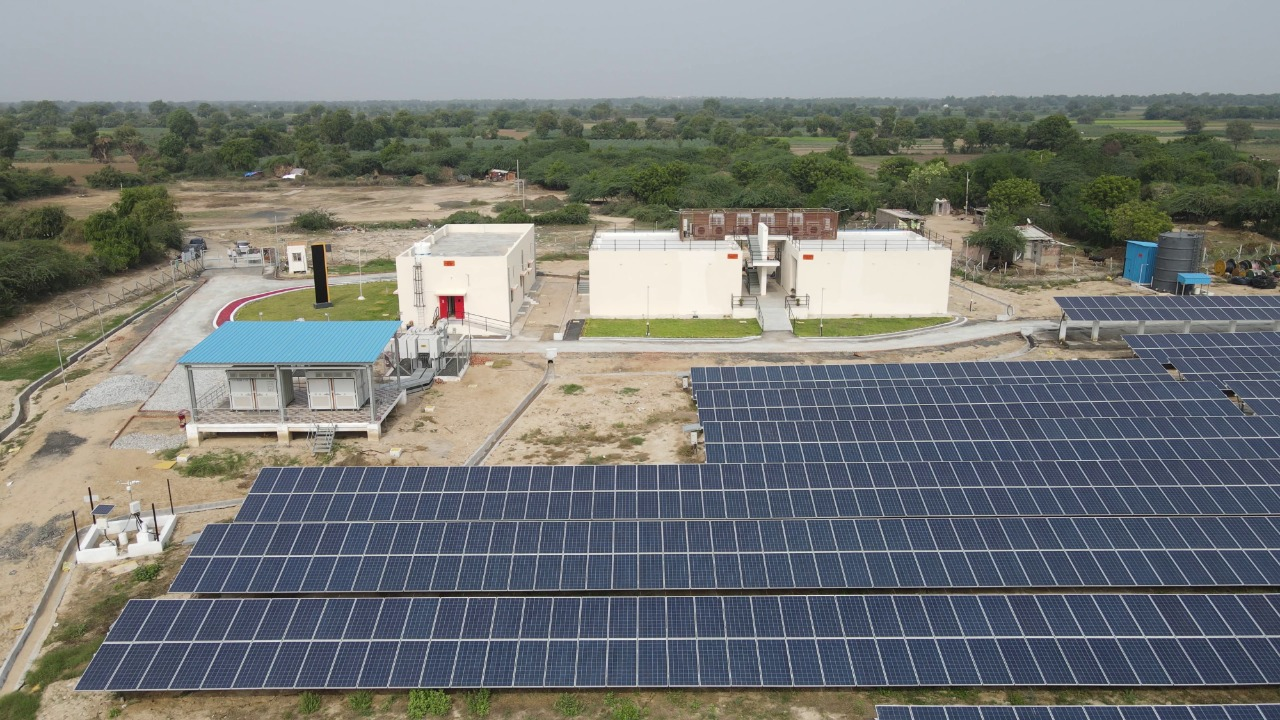
\includegraphics[width=.9\linewidth]{/Users/sainishwanth/Documents/College/Semester-6/Notes/Renewable Energy/Assignments/Modhera.jpeg}
\end{center}

\begin{quote}
“Earlier, when solar was not there, I had to pay huge amount for the electricity bill — close to 2,000 rupees. However, with the installation of the solar, my electricity bill is now zero. Everything from the refrigerator to washing machine now runs on solar in my house. I am not paying even 1 rupee electricity bill now,” - Gadvi Kailashben, Resident of Modhra.
\end{quote}


There are three main components to this project
\begin{itemize}
\item The firt is the ground mounted 6 - megawatt project
\item The second is the 15-megawatt battery storage system
\item The third is the one-kilowatt rooftops installed on 1,300 houses
\end{itemize}

The solar project not only helps with the villagers’ bills, it’s also becoming a source of income, as any surplus power they have can be sold back to the electric grid.The government buys excess energy produced here from residents if they do not use all of the capacity allotted to the households.


\begin{quote}
“We work in our farm and used to pay huge electricity bills for agriculture. Since solar installation in our village, we are now saving a lot of electricity. Earlier our electricity bill used to come around 2,000 rupees. Now it is in minus,” - Ashaben Mahendrabhai
\end{quote}

\subsection{The Idea Behid the Project}
\label{sec:orgedd0a12}
The idea behind this project is that since the Modhera temple is the Temple of the Sun God, so the entire energy of this town and community should come from solar energy,” said Mamta Verma, Principal Secretary, Energy and Petrochemicals in the Government of Gujarat.

\begin{center}
Modhera, which is associated with the Sun Temple, will also be known for its strides in solar energy.
\end{center}

\subsection{Visions for the Future}
\label{sec:orgaff2d9d}

This demonstration project is expected to provide learning to resolve bottlenecks related to renewable energy. If the project proves to be economically viable, the plan is to replicate it in other rural areas in Gujarat.

\subsection{Key Points}
\label{sec:org56fe35c}
\begin{itemize}
\item More than 1,300 households have 1 KW Rooftop Solar Systems on Residential buildings.
\item 316 KW Rooftop Solar PV Systems on various government buildings at Modhera, Samlanpura and Sujjanpura villages.
\item 6 MW Grid Connected Ground Mounted Solar PV Power Plant at Sujjanpura
\item 15 MWh, 6 MW, Battery Energy Storage System (BESS) at Sujjanpura.
\item Modhera uses only 1Mw, with rest being added to the grid.
\item Installation of Smart Energy Meters (more than 1700) at electric consumer level.
\item Fully solar-powered Sun Temple runs a 3D projection Light Show entirely on renewable energy.
\item Sensor based smart street lights near the Sun Temple.
\item 50 KW Solar Parking Infrastructure with 150 kWh Battery Storage with Electric Charging Stations at the Modhera Sun Temple.
\end{itemize}

\subsection{Other Related Initiatives}
\label{sec:org54d062a}
\begin{itemize}
\item Solar Park Scheme: The Solar Park Scheme plans to build a number of solar parks, each with a capacity of nearly 500 MW, across several states.
\item Rooftop Solar Scheme: The Rooftop Solar Scheme aims to harness solar power by installing solar panels on the roof of houses.
\item Atal Jyoti Yojana (AJAY): The AJAY scheme was launched in September 2016 for the installation of solar street lighting (SSL) systems in states with less than 50\% of households covered with grid power (as per Census 2011).
\item National Solar Mission: It is a major initiative of the Government of India and State Governments to promote ecologically sustainable growth while addressing India's energy security challenge.
\item SRISTI Scheme: Sustainable rooftop implementation of Solar transfiguration of India (SRISTI) scheme to promote rooftop solar power projects in India.
\end{itemize}

\begin{center}
India is making significant progress in the development of solar PV modules, but for it to become a manufacturing hub, it will require more policy interventions like developing home-grown technologies which could, in the short-term, work with the industry to provide them with trained human resource, process learnings, root-cause analysis through right testing and, in the long term, develop India’s own technologies.
\end{center}
\end{document}